% !TeX root = ..//diffgeo_main.tex
\begin{satz}
    Eine reguläre Kurve (das heißt $\dot{c}(t)\neq 0 \forall t \in [a, b]$) die stückweise glatt ist, ist eine Gedodätische genau dann, wenn:
    \begin{enumerate}
    \item $c$ ist eine proportional zur Bogenlänge parametrisierte Kurve
    \item Die erste Variation der Bogenlängeverschwindet für jede eigentliche Variation von $c$
    \end{enumerate}
\end{satz}
\begin{bew}
    \begin{enumerate}
        \item Sei $c$ eine Geodätische.
            Daraus folgt, dass $c$ glatt ist und nach der Bogenlänge parametrisiert ist. 
            $\Rightarrow c$ ist regulär und $\nabla_t \dot{c} = 0$. 
            Asu Gleichung für die Variation der Bogenlänge folgt:
            \begin{align*}
                &\dv{s}L(c_s)\eval{s=0} = [g(v(t), \dot{c}(t))]^b_a + \sum_i g(v(t_i), \Delta \dot{c}(t))\\
                &= 0
            \end{align*}
        \item Sei $c$ nach der Bogenlänge parametrisiert und $\partial_s L (0) = 0$ (das heißt $\dv{s}L(c_s)\eval{s=0}=0$) für jede eigentliche Variation von $c$.
            Betrachte $V = \varphi \nabla_t \dot{c}$.
            $V$ ist dann ein stückweise glattes Variationsfeld längs $c$ mit $V(t)=0$ ($t\in [a, t_i) \cup (t_{i + 1}, b]$)
            Bilde eigentliche Variation $c_s$ von $c$ mit Variationsfeld $V$.
            \begin{align}
                \label{eq:sollverschw}
                0 = \partial_s L(0) &= - \int^{t_{i + 1}}_{t_i} g(\varphi \nabla_t \dot{c}, \nabla_t \dot{c}) \dd t\\
                &= - \int^{t_{i+1}}_{t_i} \varphi \norm{\nabla_t \dot{c}} \dd t
            \end{align}
            Daraus folgt, dass $\norm{\nabla_t \dot{c}} = 0$.
            Damit folgt, dass $c\eval{[t_i, t_{i+1}]}$ eine Geodätische ist.
    \end{enumerate}
    Wir wollen nun noch ein Argument angeben, warum Gleichung \ref{eq:sollverschw} verschwindet.
    Setze $f(t_i) = \dot{c}(t_i - 0) - \dot{c}(t_i - 0)$ und betrachte das parallele Vektorfeld $F$ längs $c$.
    Setze $V = \varphi F $ und betrachte die zugehöreige Einparameter Variation von $c$.
    Dann gilt:
    \begin{align*}
        0 &= \partial_s L(0) = g(v(t_i), \dot{c}(t_i - 0) - \dot{c}(t_i - 0))\\
        &= \varphi(t_i) g(f(t_i), f(t_i))
    \end{align*}
\begin{align}
    f(t_i) = \dot{c}(t_i - 0) - \dot{c}(t_i + 0) = 0
\end{align}
\end{bew}
\section{$(\mfk, g)$ als metrischer Raum} 
Ziel sit es jetzt zu zeigen, dass $(\mfk, d)$ ein metrischer Raum ist, wobei $d$ eine geeignet definierte Distanzfunktion ist.
Um dieses Ziel zu erreichen, benötigen wir zunächst ein paar Überlegungen zur Exponentialabbildung.
Die Exponentialabbildung hat die folgende geometrische Eigenschaft.\\
\missingfigure{Exponentialabbildung}
Es ist zu sehen, dass der Strahl $t v$ auf radiale Geodätische $c_v(t) = \exp_p (t v)$ abgebildet.
$\exp_p$ erhält Orthogonalität zu den radialen Richtungen.
Dies nennt man \textbf{radiale Isometrie}.
\begin{lem}[Gaußlemma]
    \label{lem:gaußlemma}
    Sei $p \in \mfk$, $v \in T_p \mfk $ und $c_v(t) = \exp_p(tv)$ auf $[0, b]$ definiert.
    Dann ist $\exp_p$ in einer offenen Umgebung von $\{ tv \vert t\in [a, b] \} \subset T_p \mfk$ definiert und es gilt.
    \begin{itemize}
     \item[a)] $\dd ( \exp_p \eval{t v})(v) = \dot{c}_v(t)$
    \item [b)] Für $\eta \in T_{tv} ( T_p \mfk ) \cong T_p \mfk$ gilt:
    \begin{align*}
        g(d(\exp_p)_{tv} (\eta), d(\exp_{tv})(v)) = g(\eta, v)
    \end{align*}
    \end{itemize}
\end{lem}
\begin{bew}[Beweis Gaußlemma \ref{lem:gaußlemma}]
zu a):
\begin{align*}
    \dd(\exp_p\eval_{tv})(v) &= \dv{s}\eval_{s=0} \underbrace{\exp_p (tv + sv )}_{c_v(t+s)}\\
    &= \dv{s} \eval_{s=0} c_v (t+s) = \dot{c}_v (t)\\
    &= \dot{c}_c (t)
\end{align*}
zu b):\\
Wir können ohne Beschränkung der Allgemeinheit annehmen, dass $t=1$ (da $c_{tv}(1) = c_v (t)$).
Ferner betrachten wir die Variation $H$ von $c_v$:
\begin{align*}
    &H: (-\varepsilon, \varepsilon)\times[0, 1] \to \mfk\\
    & H(s, t) = \exp_p (t(v + s \eta))
\end{align*}
$V(t)$ sei das zugehörige Variationsfeld mit
\begin{align*}
    V(t) = \dv{s} \eval_{s=0} H(s,t)
\end{align*}
Außerdem ist $c_s(t) = \exp_p (t(v+s\eta))$.
\begin{align*}
    &L(c_s) = \sqrt{g(v + s \eta, v + s \eta)}\\
\end{align*}
\begin{align}
    \label{eq:variation1}
\Rightarrow \partial_s L(0) = \frac{1}{\norm{v}}g(v, \eta)      
\end{align}
Wir können $\partial_s L(0)$ auch mittels der ersten Variation der Bogenlänge berechnen.
\begin{align} 
\partial_s L (0) &= \frac{1}{\norm{v}} g(v(t), \dot{c}_v (t))\eval^1_0\\
&= \frac{1}{\norm{v}} (g(v(1), \dot{c}_v (1)) - g(v(0), \dot{c}_v (0)))\\
\label{eq:variation2}
&= \frac{1}{\norm{v}} (g(d(\exp_p)\eval_v (\eta), \dot{c}_v(1)) - g(v(0), \dot{c}_v (0)))
\end{align}
Die Gleichungen \ref{eq:variation1} und \ref{eq:variation2} implizieren die Behauptung, falls
\begin{align*}
    g(v(0),\dot{c}_v (0)) = 0
\end{align*}
ist.\\
Nach a) können wir ohne Beschränkung der Allgemeinheit annhmen, dass $\eta \perp v$ ist (Warum?).
Das heißt:
\begin{align*}
    0 &= g(\eta, v) = g(\eta, \dot{c}_v(0))\\
    &= g(v(0), \dot{c}_v (0))
\end{align*}
\end{bew}

\begin{defs}[Distanzfunktion]
    Seien $p, q \in \mfk$, so ist
    \begin{align}
        \label{eq:distanzfuntion}
        d(p,q) := \inf \{ L(c) \vert c : [a, b]\to \mfk \ \text{Stückweise glatt mit} \ c(a) = p \ \text{und} \ c(b) = q \}
    \end{align}
    die Distanzfunktion.
\end{defs}
\begin{bsp}
Im $\R^2$ wäre die Distanz zwischen den Punkten $p$ und $q$ die Länge der roten Kurve (Gerade) in Abbildung \ref{img:variation}
\begin{figure}[H]
\centering
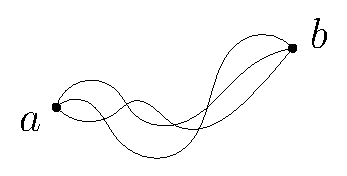
\includegraphics[width=0.3\linewidth]{figures/tikz/variation.pdf}
\caption{Variation}
\label{img:variation}
\end{figure} 
\end{bsp}


\begin{bem}\leavevmode
    \begin{itemize}
        \item Infimum muss nicht angenommen werden (Beispiel: $\R^2 \backslash 0 $)
        \item Die Kürzeste Strecke ist im Allgemeinen nicht eindeutig.
     \end{itemize}
\end{bem}
